\chapter{Model}
\label{chap:model}

\section{Introduction}
\label{sec:introduction}
In this chapter a technical description of the implemented model will be given.\par 
Firstly, a description of the dataset will be given. Furthermore, the data munging preprocessing will be made clear. Later on, the model building alongside with the classificator options shall be extensively explained, making emphasis on the best classificator results. Finally, the parameter optimization will be briefed altogether with the best founded parameters results.
\section{Dataset}
\label{sec:use-cases}
This section explains the dataset choice, as well as the main label present in the dataset.\par
This project is fromerly designed to detect sarcasm in spanish written texts, more particularly tweets. Therefore, all the datasets used in this project are written in spanish.\\
The dataset body will contain two rows, the tweet body, i.e. the text, and a binary value expressing the sarcasm nature of that tweet.\\
The entire body of the dataset is composed of three datasets. The initial database ~\cite{mexic} consists of 4529 sarcastic tweets and 335 non-sarcastic tweets. Even though 4529 labelled tweets is a good start, the dataset is completely unbalanced. Consequently, new tweets had to be searched to obtain a properly balanced dataset. Considering the fact that the mayority of the dataset is sarcastic, finding new non-sarcastic tweets is not a difficult duty.\\
At the end, the result was 5638 sarcastic tweets and 5444 non-sarcastic. That can be rewritten as $49.12\%$ of non-sarcastic and $49.5\%$ of sarcastic tweets.\par

The ~\cref{fig:dataset} displays the dataset structure. As explained before, there is one column showing the tweet text and another column showing the sarcastic value of the tweet. The '1' refers to sarcastic, while '0' is non-sarcastic.
\begin{figure}
	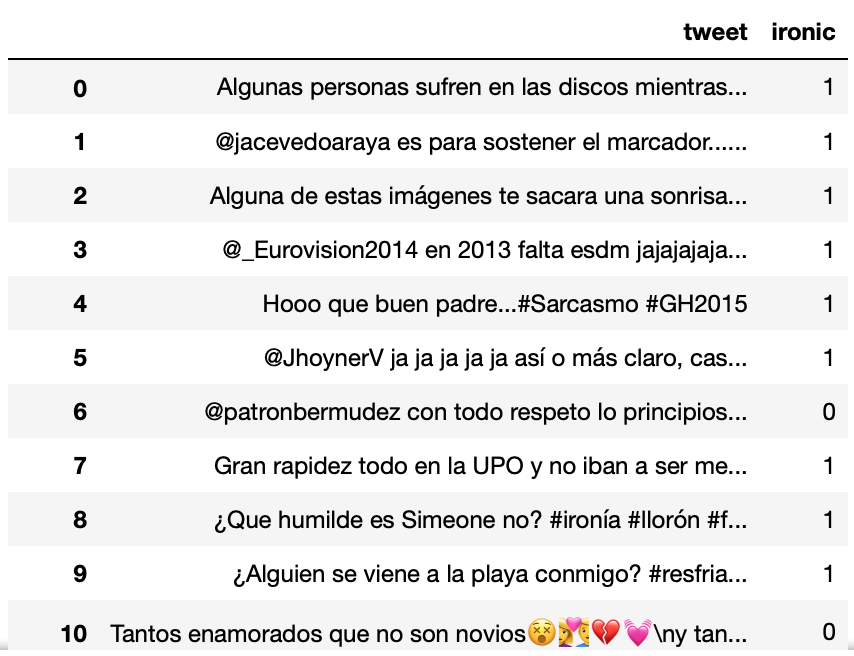
\includegraphics[width=\linewidth]{img/dataset.png}
	\caption{Dataset}
	\label{fig:dataset}
\end{figure}

\section{Preprocessing}
\label{sec:preprocessing}
The preprocessing stage is conceived to dispose of any information that will not be needed during the \ac{ml} step ~\cite{preprocess}. The preprocessing was applied individually to each tweet.
The changes in the dataset that have been made are:
\begin{itemize}
	\item \textit{False items}: Since almost half the dataset tweets come from tweeter, it was required to download those tweets from the social network. Some of the captured tweets were false.
	\item \textit{Categorical values}: Originally the labels of the dataset were either 'True' or 'False'. These two values were encoded into 'True'= 1 and 'False' = 0.
	\item \textit{Stopwords}: In \ac{ml} it is very common to delete words which provide barely no information to the text (e.g. 'a', 'I', 'you'). In this project, the list of stopwords was chosen for the spanish language. The list of words can be consulted in ~\cite{stopwords}.
	\item \textit{Tokenization}:This process consists of splitting a string (tweet) into tokens.
	\item 
	\textit{Stemming}: This process cosnists of reducing the tokens into its root. Stemming was accomplished using a Snowball stemmer. 
\end{itemize}
These steps of preprocessing were all executed defining a custom tokenizer but the categorical value encoding and the false item removal, which were done previously.\\
It is noteworthy to mention that the custom tokenizer is used later for the feature extraction. 
